\documentclass[12pt,a4paper]{report}
\setlength\textwidth{145mm}
\setlength\textheight{247mm}
\setlength\oddsidemargin{15mm}
\setlength\evensidemargin{15mm}
\setlength\topmargin{0mm}
\setlength\headsep{0mm}
\setlength\headheight{0mm}
\setlength{\parindent}{4em}

\let\openright=\clearpage


\usepackage[czech]{babel}

\usepackage[utf8]{inputenc}

\usepackage{indentfirst}
\usepackage{graphicx}
\usepackage{color}
\usepackage{pdfpages}

\usepackage{amsthm}
\usepackage{setspace}

\usepackage[unicode]{hyperref}  
\hypersetup{pdftitle=Název práce}
\hypersetup{pdfauthor=Jméno Příjmení}


\makeatletter
\def\@makechapterhead#1{
  {\parindent \z@ \raggedright \normalfont
   \Huge\bfseries \thechapter. #1
   \par\nobreak
   \vskip 20\p@
}}
\def\@makeschapterhead#1{
  {\parindent \z@ \raggedright \normalfont
   \Huge\bfseries #1
   \par\nobreak
   \vskip 20\p@
}}
\makeatother


\def\chapwithtoc#1{
\chapter*{#1}
\addcontentsline{toc}{chapter}{#1}
}

\begin{document}


\lefthyphenmin=2
\righthyphenmin=2


\pagestyle{empty}
\begin{center}

\large

{ \bf ČESKÁ ZEMĚDĚLSKÁ UNIVERZITA V PRAZE}

\medskip

FAKULTA ŽIVOTNÍHO PROSTŘEDÍ

\medskip

{\sc \Large katedra vodního hospodářství a~environmentálního modelování}

\vfill

\vfill

{\LARGE Vizualizace enviromentálních dat}

\vspace{2mm}

{\bf \Large BAKALÁŘSKÁ PRÁCE}

\vspace{15mm}

\vfill

\vfill

\begin{tabular}{rl}

\noalign{\vspace{2mm}}
Vedoucí práce: & \bf doc. Ing. Martin Hanel, Ph.D. \\
\noalign{\vspace{2mm}}
Bakalant: & \bf Irina Georgievová \\
\end{tabular}

\vfill

2018

\end{center}
\newpage
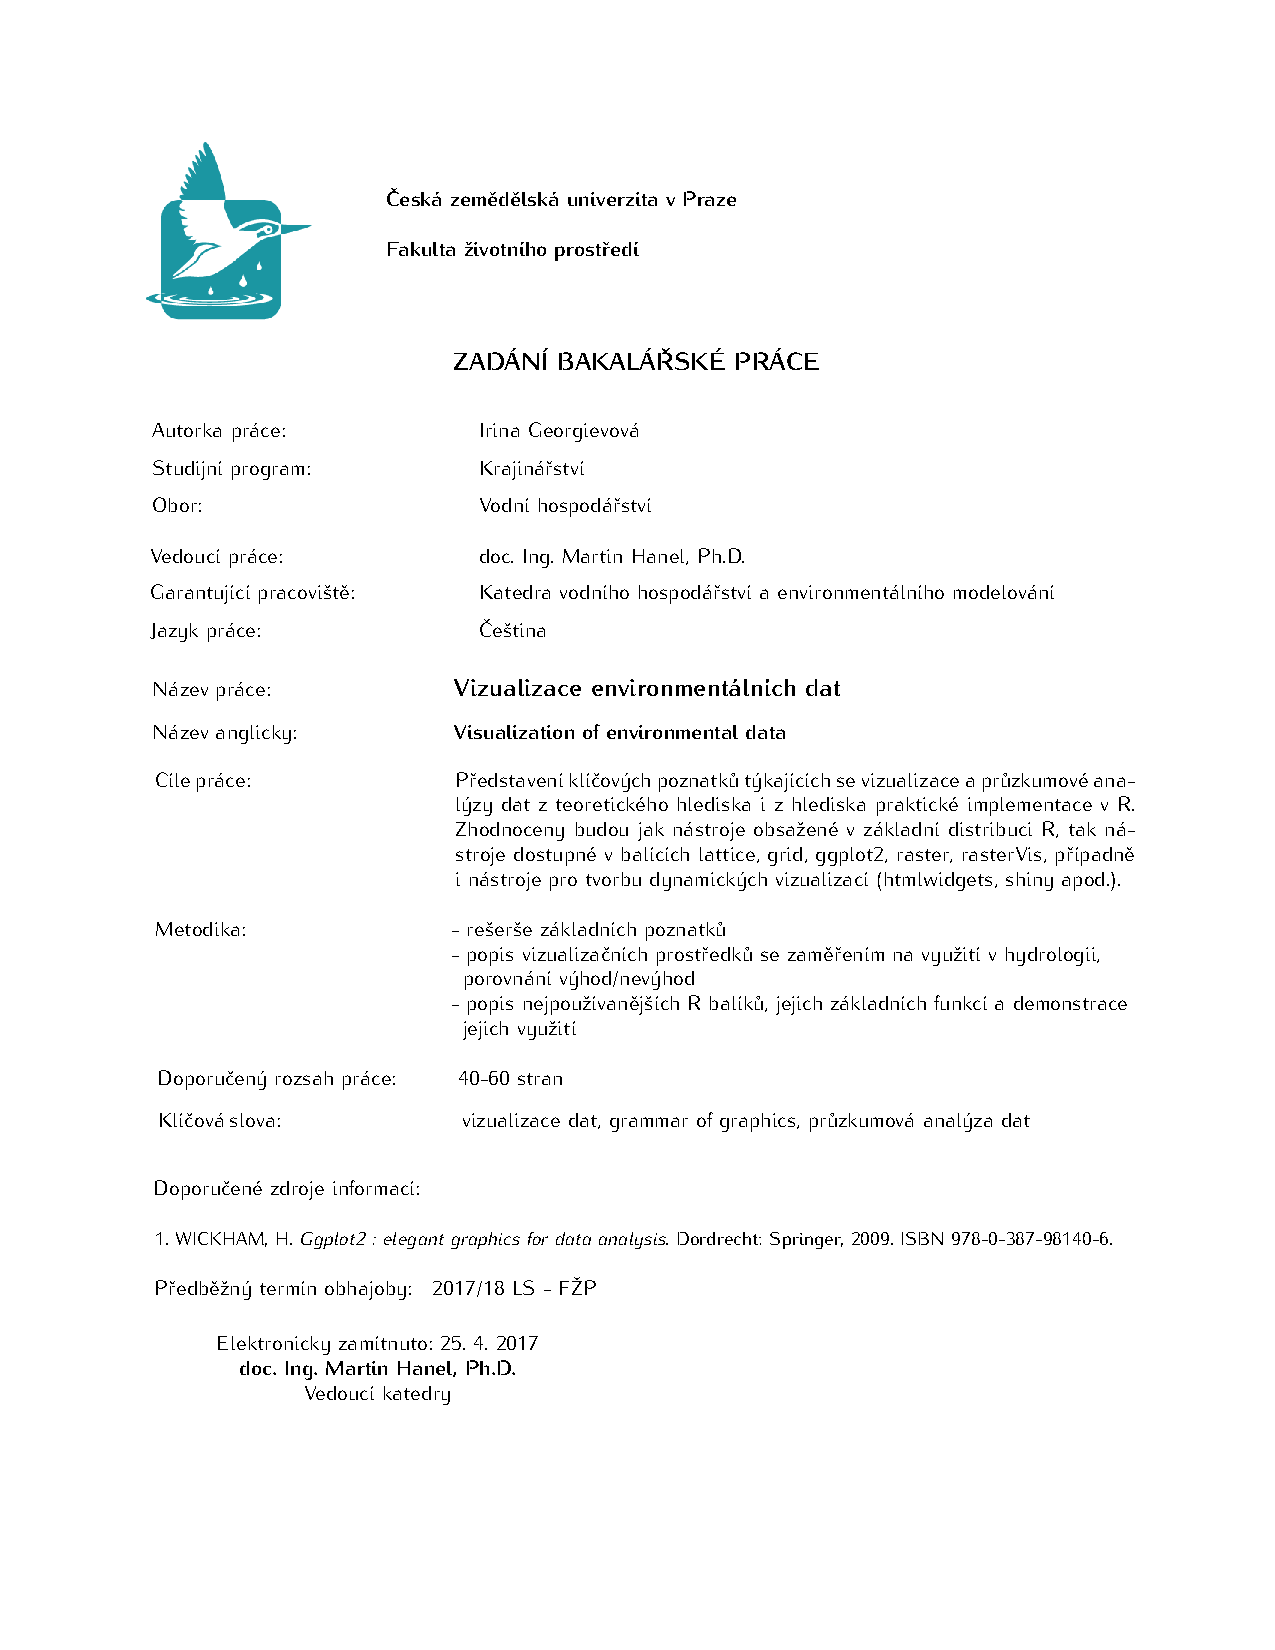
\includepdf[pages={1,2},pagecommand={}, scale = 0.75]{zadani.pdf}
\newpage


\vglue 0pt plus 1fill

\noindent
{\bfseries Prohlášení:} \\

Prohlašuji, že jsem bakalářskou práci \emph{Vizualizace enviromentálních dat} zpracovala samostatně. Veškerou literaturu a další podkladové materiály uvádím v~ seznamu na straně ~\pageref{literatura}. \\

Prohlašuji, že tištěná verze se shoduje s verzí odevzdanou přes Univerzitní informační systém.

\vspace{10mm}

\hbox{\hbox to 0.5\hsize{%
V Praze dne ..................
\hss}\hbox to 0.5\hsize{%
\hspace{100pt}...........................
\hss}}

\vspace{1mm}
\hbox{\hbox to 0.5\hsize{%

\hss}\hbox to 0.5\hsize{%
\hspace{100pt}Irina Georgievová
\hss}}

\vspace{20mm}

\newpage

\vglue 0pt plus 1fill
\noindent
{\bfseries Poděkování:} \\

Ráda bych poděkovala doc. Ing. Martinu Hanelovi, Ph.D. za cenné rady, věcné připomínky a vstřícnost při konzultacích a při vypracovávání bakalářské práce.

\newpage

\newpage


\vbox to 0.5\vsize{
\setlength\parindent{0mm}
\setlength\parskip{5mm}

{\LARGE\bfseries Abstrakt} 

Vizualizace je klíčovým nástrojem pro přehlednou a srozumitelnou prezentaci dat a jejich průzkumovou analýzu, kde přispívá k odhalení nečekaného chování dat a~k~dalšímu rozhodování o směru analýzy. Práce shrnuje historii vývoje vizualizace dat a~její teorii, jejíž vědecké základy byly položeny především Williamem S. Clevelandem, Edwardem Tuftem a Lelandem Wilkinsonem. Dále práce popisuje současné nástroje vizualizace dat v programovacím jazyku R a probírá, jak základní, tak i pokročilé vizualizační balíčky (\texttt{grid}, \texttt{lattice}, \texttt{ggplot2}, \texttt{raster} a další). Hlavním přínosem práce je vytvoření webové aplikace pomocí nástrojů pro interaktivní vizualizaci (\texttt{htmlwidgets}, \texttt{Shiny} a \texttt{flexdashboard}).  Aplikace je určena pro usnadnění analýzy hydrologické bilance a předpovědí sucha v útvarech povrchových vod České republiky a demonstruje výhody moderní vizualizace dat. 

{\bfseries Klíčová slova: } vizualizace dat, grammar of graphics, průzkumová analýza dat, R, Shiny
\vss}\nobreak\vbox to 0.49\vsize{
\setlength\parindent{0mm}
\setlength\parskip{5mm}
{\LARGE\bfseries Abstract} 

Visualization is a key tool for a clear and comprehensive presentation of data and their exploratory analysis, where it helps to discover unexpected data behavior and to further decide on the analysis direction. This thesis summarizes the history of development of data visualization and its theory, whose scientific base was laid mainly by William S. Cleveland, Edward Tuft and Leland Wilkinson. The thesis also describes current data visualization tools in programming language R and discusses both basic and advanced visualization packages (\texttt{grid}, \texttt{lattice}, \texttt{ggplot2}, \texttt{raster} and others). The main contribution of this thesis is development of a web application which uses interactive visualization tools (\texttt{htmlwidgets}, \texttt{Shiny} and \texttt{flexdashboard}). The application is designed to facilitate analysis of hydrological balance and drought prediction of surface water bodies of the Czech Republic and demonstrates the advantages of modern data visualization.

{\bfseries Keywords:  } data visualization,  grammar of graphics, exploratory data analysis, R, Shiny
\vss}

\end{document}
